\documentclass[sigconf,nonacm]{acmart}
\settopmatter{printacmref=false,printfolios=true}
\setcopyright{none}
\renewcommand\footnotetextcopyrightpermission[1]{}
\usepackage{amsmath,tabularx,array,enumitem,balance}
\usepackage{graphicx}
\usepackage{tikz}
\usetikzlibrary{arrows.meta,positioning}
\definecolor{CourseBlue}{HTML}{315EFB}
\definecolor{CourseTeal}{HTML}{14877D}
\hypersetup{colorlinks=true,linkcolor=CourseBlue,citecolor=CourseTeal,urlcolor=CourseTeal}
\newcolumntype{Y}{>{\raggedright\arraybackslash}X}
\setlist{leftmargin=*,topsep=2pt,itemsep=1pt}

%% Week 2 agenda maps the seven parallel sessions one-to-one onto the seven
%% teams (Session A = Team 1 ... Session G = Team 7).  Team 7 -> Session G.
\newcommand{\WorkshopSession}{Session G (Team 7)}

\newcommand{\CourseNumber}{COMSCI/ECON 206}
\newcommand{\CourseName}{Computational Microeconomics}
\newcommand{\CourseSession}{Autumn 2026 Session 1}
\newcommand{\Instructor}{Luyao Zhang}

%% Artifact links. CommitHash names the commit holding the code and results that
%% produced every number in Sections 3-4; later commits only touch prose.
\newcommand{\GitHubLink}{https://github.com/24hours68435790-cmd/PS1-Feiyu}
\newcommand{\ColabLink}{https://colab.research.google.com/github/24hours68435790-cmd/PS1-Feiyu/blob/main/companion/notebooks/PS1\_strategic\_disclosure.ipynb}
\newcommand{\CommitHash}{1081926}
\newcommand{\DemoLink}{https://huggingface.co/spaces/24hours6964/strategic-disclosure-game}

\newcommand{\coursemeta}{\noindent\footnotesize\textbf{Submission to:} \CourseNumber{} --- \CourseName.
\textbf{Course session:} \CourseSession. \textbf{Workshop:} \WorkshopSession.
\textbf{Instructor:} \Instructor. \textbf{Assignment:} PS1 research proposal, v2.
\textbf{Artifacts:} \url{\GitHubLink} $\cdot$ \url{\ColabLink} $\cdot$ \url{\DemoLink}\par\smallskip}

\title{When the Model Becomes the Target: Strategic Disclosure under AI-Assisted Valuation}
\author{Feiyu Li}
\affiliation{\institution{Duke Kunshan University}\city{Kunshan}\country{China}}
\email{feiyu.li@dukekunshan.edu.cn}
\renewcommand{\shortauthors}{Feiyu Li}

\begin{document}

\begin{abstract}
When an AI model prices firms on their own reported metrics, the metric becomes
a target. Can an evaluator that \emph{remembers} a firm substitute for one that
\emph{commits} to a fixed rule? Following the distinction Banchio et al.\ draw
for auctions between an announced rule and the rule a designer follows, I compare
a \textsc{committed} evaluator against a \textsc{revisable} one on an identical
two-period tree, so only the rule differs. A Python twin of the deployed browser
Space reproduces its logged prices to the cent, then sweeps what a browser
cannot. Memory halves the gain from inflating, but only in rounds with a
successor, and it prices an honest firm below value once outcome noise exceeds
the announced allowance. All results are simulated outputs of my own model.
\end{abstract}

\keywords{strategic disclosure, credible rules, AI valuation}

\begin{teaserfigure}
\centering
%% The figure is built wide and flat (~21 x 2.2 cm) precisely so it can run at
%% full width and still cost only ~2 cm of height -- see the design note in
%% figures/ps1_teaser_body.tex. Do NOT shrink this to fit; uniform scaling
%% would take the 7pt labels down with it. Cut prose instead.
\resizebox{\textwidth}{!}{%% Teaser figure body -- ONE source of truth.
%% Included by main.tex (inline, no external PDF) and by ps1_teaser.tex (standalone).
%% Requires: tikz + libraries arrows.meta, positioning; colours CourseBlue, CourseTeal.
%%
%% DESIGN NOTE -- why this is wide and flat, and why the width is pinned.
%% \resizebox scales uniformly, so the vertical space this costs on the page is
%%     display width  x  (natural height / natural width),
%% and every label is scaled by  (display width / natural width).
%% Natural size here is ~21.4 x 2.5 cm (aspect ~8.6:1). Run at \textwidth it
%% costs ~2.1 cm of height while the scale factor stays near 0.83, so the 7pt
%% labels land near 5.8pt. An earlier 17 x 6.8 cm layout had to be shrunk to
%% 0.22\textwidth to fit, which rendered those labels at 1.6pt.
%%
%% Two competing constraints fix the width near 21 cm:
%%   - WIDER  -> every label shrinks (scale = 17.8 / natural width).
%%   - NARROWER -> the H1-H3 line no longer fits on two lines.
%% To save more height, shorten the box text or the H1-H3 parentheticals.
%% Do NOT shrink the \resizebox in main.tex.
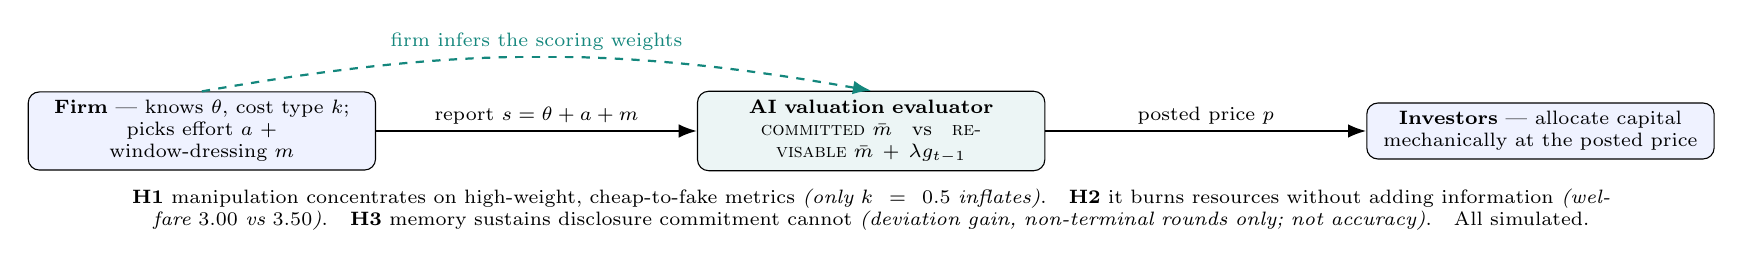
\begin{tikzpicture}[
  >=Latex,
  box/.style   = {draw, rounded corners, align=center, text width=42mm,
                  inner sep=3pt, font=\scriptsize},
  lbl/.style   = {font=\scriptsize, align=center, inner sep=2pt, fill=white},
  arrow/.style = {->, thick},
  darrow/.style= {->, thick, dashed, CourseTeal}
]

%% ---- one flat row: firm -> evaluator -> investors ---------------------
\node[box, fill=CourseBlue!8] (firm) at (0,0)
  {\textbf{Firm} --- knows $\theta$, cost type $k$;\\
   picks effort $a$ + window-dressing $m$};

\node[box, fill=CourseTeal!8] (eval) at (8.5,0)
  {\textbf{AI valuation evaluator}\\
   \textsc{committed} $\bar m$\;\; vs\;\; \textsc{revisable} $\bar m+\lambda g_{t-1}$};

\node[box, fill=CourseBlue!8] (inv) at (17,0)
  {\textbf{Investors} --- allocate capital\\
   mechanically at the posted price};

\draw[arrow] (firm) -- node[lbl, above] {report $s=\theta+a+m$} (eval);
\draw[arrow] (eval) -- node[lbl, above] {posted price $p$} (inv);

%% ---- the channel that makes the loop strategic ------------------------
%% Shallow arc (out/in = 10 deg) so the bounding box stays flat.
\draw[darrow] (firm.north) to[out=10, in=170]
  node[lbl, above, pos=0.5] {firm infers the scoring weights} (eval.north);

%% ---- hypotheses: 205mm box, text trimmed to wrap to exactly TWO lines -
\node[font=\scriptsize, align=center, text width=205mm] at (8.5,-1.0)
  {\textbf{H1} manipulation concentrates on high-weight, cheap-to-fake metrics
   \emph{(only $k=0.5$ inflates)}.\quad
   \textbf{H2} it burns resources without adding information
   \emph{(welfare $3.00$ vs $3.50$)}.\quad
   \textbf{H3} memory sustains disclosure commitment cannot
   \emph{(deviation gain, non-terminal rounds only; not accuracy)}.\quad
   All simulated.};

\end{tikzpicture}
}
\caption{A firm privately knowing $\theta$ and cost type $k$ picks effort $a$
and window-dressing $m$; the evaluator either \textsc{commits} to the announced
$\bar m$ or \textsc{revises} to $\bar m+\lambda g_{t-1}$ from this firm's own
history---the wedge Banchio et al.\ identify in auctions~\cite{banchio2025}.
Section~3 switches only that box. Simulated.}
\Description{A wide left-to-right diagram with three boxes in a single row. The
Firm, which privately knows quality theta and cost type k and picks effort and
window-dressing, sends a report s to the AI valuation evaluator. The evaluator
box states two alternatives: a committed rule that follows the announced
allowance, and a revisable rule that follows the allowance adjusted by lambda
times the residual read off this firm's own history. The evaluator posts a price
to Investors, who allocate capital mechanically. A dashed arc above the row shows
the firm inferring the scoring weights.}
\label{fig:teaser}
\end{teaserfigure}

\maketitle\raggedbottom\coursemeta

\section{Three connected research questions}
Algorithmic scoring makes reported firm metrics consequential for capital
allocation, and once a metric is a target the firm optimises the number rather
than the fundamentals behind it~\cite{strathern1997}. Economics has studied this
against human markets for decades---earnings management~\cite{healy1999},
signal-jamming~\cite{stein1989}, funds inflating interim returns around
fundraising~\cite{brown2019}---and machine learning arrives from the other side:
a deployed model changes the distribution it predicts~\cite{perdomo2020} and
agents respond to the announced rule~\cite{hardt2016}. The stakeholders are the
firms being scored, investors allocating mechanically from the posted price, and
an auditor who observes the evaluator's behaviour but not its weights.

\textbf{The strategic tension.} An AI evaluator, unlike a market, can retrain,
so it need not follow the rule it announces. That is where the 2001 Nobel
foundation stops~\cite{nobel2001}: costly signals carry information under
unequal information~\cite{spence1973}, but the receiver's rule is fixed. Two
recent results suggest an alternative discipline---cooperation emerges from
opponent-specific responses in repeated dilemmas~\cite{morozov2026} and remains
learnable under minimal observability~\cite{leung2026}---while Banchio,
Skrzypacz and Yang show, for auctions, that credibility is the gap between an
announced rule and the rule the designer will actually
follow~\cite{banchio2025}. I transplant that distinction to valuation;
Figure~\ref{fig:teaser} is the resulting loop.

\begin{itemize}
\item \textbf{Q1---Economics.} When an evaluator can revise its rule, does
opponent-specific memory discipline disclosure the way commitment does, and at
what cost in allocative efficiency?
\item \textbf{Q2---Computation.} Can such a rule be made comparable and
auditable---encoded as a finite game, run against a fixed rule on identical
draws, and rechecked by someone with neither the weights nor the data?
\item \textbf{Q3---Behaviour.} Is the manipulation cost that makes memory work a
real property of reporting officers, or an artefact of assuming convexity?
\end{itemize}

They are not separable: Q1's answer is a function of the cost distribution Q3
supplies, Q3's test is interpretable only inside the game Q1 specifies, and Q2
is what lets a third party check either. \textbf{Integrated question: when firms
know the metrics an AI valuation model uses, under what conditions can an
evaluator that remembers a particular firm substitute for one that commits to a
fixed rule---and when does remembering instead punish the honest?}

\section{Answer to Q1: incentives and intellectual lineage}
\textbf{Provisional answer (falsifiable).} Memory substitutes for commitment on
the \emph{deterrence} margin, not on accuracy, and only in rounds that have a
successor.

\textbf{Players, actions, payoffs, timing, information.} A firm privately knows
quality $\theta\in\{1,2,3\}$ and manipulation-cost type $k\in\{0.5,1,2\}$; an
evaluator prices; investors allocate mechanically and are not strategic. Per
round the firm picks effort $a\in\{0,1\}$ and window-dressing $m$ on a grid and
reports $s=\theta+a+m$. A \emph{strategy} maps the type into a pair of actions
across two rounds---which is why $m_1$ and $m_2$ can differ for one type though
the \emph{action} set is identical. Payoffs: firm
$\pi=p-0.5a-km^{2}$; welfare $W=v-km^{2}$ with $v=\theta+a$; the evaluator is
scored by $|p-v|$. Timing: the firm reports, the evaluator posts $p$, and only
then is $y=v+\epsilon$ realised. Information: $\theta$, $k$ and $\epsilon$ are
unobserved by the evaluator; the allowance $\bar m$ is announced. Solution
concept: perfect Bayesian equilibrium in the sense Harsanyi
defined~\cite{harsanyi1968}. The course-scale computation reports type-by-type
best responses against a posted rule rather than a full fixed point---a
limitation stated here so it is not read as a result.

\textbf{The two rules.} \textsc{Committed}: the announced $\bar m$ is the one
followed, every round, every firm. \textsc{Revisable}: $\bar m$ is still
announced, but after round~1 the evaluator follows $\bar m+\lambda g_1$, where
$g_1=(s_1-y_1)-\bar m$ is the residual inflation it can infer. That wedge
between announced and followed is the Banchio et al.\ object~\cite{banchio2025},
moved from auction design to valuation.

\textbf{Benchmark and evidence status.} Frankel and Kartik establish that
\emph{committing} to underuse manipulable data can improve
allocation~\cite{frankel2022}; they leave open what a receiver that can retrain
should do. $\theta$, $k$, $\bar m$, $\lambda$ and $\epsilon$ are hypothetical
model primitives; every number in Section~3 is an observed output of my own
simulation; cost convexity is \emph{inherited} as motivation
from~\cite{fischbacher2013}, never estimated; nothing comes from firm data.

\section{Answer to Q2: method and evaluation}
\textbf{Inputs, algorithm, baseline, metric.} Inputs are
$(\theta,k,\sigma,\lambda)$ and the action grid. The algorithm enumerates every
two-round strategy and takes expected payoff over 20{,}000 draws of
$\epsilon\sim U(-\sigma,\sigma)$. The baseline is \textsc{committed}; the single
modification makes the rule \textsc{revisable}. Following the instructor's
Week~2 note I record \emph{disclosure accuracy} (mean $|p-v|$) \emph{and
deviation gain}---the expected payoff of the best strategy minus that of
reporting honestly at the same effort---alongside welfare.

\textbf{The meaningful check.} The notebook re-implements JavaScript's
\texttt{mulberry32} PRNG in Python and reproduces all four cases logged from the
deployed Space---same draw ($\theta=2$, $k=0.5$), same $\epsilon$ sequence, same
prices, to the cent---as an assertion, so the run fails rather than quietly
disagrees. Game and notebook are therefore the \emph{same} model, and the page
exposes the same two knobs, so a reader reaches the Section~4 threshold by hand
(seed~2, $\sigma=2$: an honest firm priced 2.00 against true value 4.00, where
commitment says 3.00). One scope difference is not hidden: the page draws
$\epsilon$ from $\{-\sigma,0,+\sigma\}$ and the notebook from
$U(-\sigma,\sigma)$, so mis-punishment \emph{frequency} differs ($2/3$ versus
$(\sigma-\bar m)/\sigma$) though the threshold $\sigma^{*}=\bar m$ does not.

\textbf{Obtained} (simulated outputs of my own model, not evidence about any real
firm; averaged over all nine types).
\begin{itemize}
\item \emph{Deviation gain halves} under \textsc{revisable}---$0.333\to0.167$ on
the browser grid, $0.692\to0.346$ on the research grid---and is flat in $\sigma$
across $[0,3]$. This is the margin on which H3 survives.
\item \emph{Deterrence stops at the horizon.} The cheap type ($k=0.5$) sets
$m_1=0$ under \textsc{revisable} but still $m_2=1$: memory disciplines every
round that has a successor, and no more.
\item \emph{Accuracy moves the other way on every grid} ($0.750$ vs $0.667$
browser; $0.869$ vs $0.571$ research), because the revisable round-2 price
carries the noise while commitment deducts a constant. Welfare runs opposite on
both ($5.833$ vs $5.667$; $5.632$ vs $5.263$): commitment buys precision with
burnt resources, reaching $|p-v|=0$ for the $k=0.5$ type only by inducing
exactly the inflation it allows.
\item \emph{The coarse grid distorts the honest share}---two-thirds read as
fully honest under both rules, against $0.000$ on the research grid, because a
finer $m$ grid always leaves a profitable small inflation. This is the
grid-sensitivity check v1 promised and never ran, and it is why H3 is stated on
deviation gain and welfare---magnitudes that survive the grid change---not on a
binary split.
\end{itemize}

\textbf{Planned, not obtained.} A CFR fixed point in
OpenSpiel~\cite{lanctot2019} on the identical tree; horizons beyond two;
heterogeneous evaluators.

\section{Answer to Q3: behaviour and competing explanations}
\textbf{Mechanism and its competitor.} The model assumes a convex, privately
known manipulation cost---the behavioural reading of die-roll evidence that
honesty is heterogeneous, with partial liars alongside honest and fully
self-serving reporters~\cite{fischbacher2013}. The competing explanation is that
reporting officers pay no such cost but reason boundedly: they do not compute
that a revisable evaluator prices the inflation out next round, so what looks
like cost is a reasoning limit~\cite{wright2020}.

\textbf{Evidence that discriminates.} The two predict opposite things about
$\lambda$: a cost story predicts \emph{saturation} once anticipated punishment
exceeds the gain, bounded reasoning predicts continued response to more visible
punishment. The sweep shows saturation---deviation gain falls
$0.333\to0.250\to0.167$ as $\lambda$ goes $0\to0.25\to0.5$, then is flat to
$\lambda=2$---while mispricing is minimised at $\lambda=0.25$ and rises
thereafter. \textbf{The $\lambda=1$ hard-coded in my v1 demo therefore buys no
deterrence over $\lambda=0.5$ and costs accuracy}; both optima are interior and
they differ. The feasible next test is a within-subject reporting experiment
varying $\lambda$ while eliciting beliefs about the next-round price.

\textbf{Can memory punish the honest?} Yes, with a threshold. An honest firm
($m=0$) is priced below true value in $49.9\%$ of draws for every $\sigma>0$,
but \emph{worse than under commitment} only once $\sigma>\bar m$, with share
$(\sigma-\bar m)/\sigma$: simulation returns $0.198$, $0.331$, $0.500$, $0.668$
at $\sigma=1.25,1.5,2.0,3.0$ against an analytic $0.200$, $0.333$, $0.500$,
$0.667$; on the mean the crossing comes at $\sigma=2\bar m$. Disparate-impact
risk is therefore bounded by noise over announced allowance---and small, young
firms are precisely those with noisy outcomes, which makes that ratio what a
regulator would need.

\textbf{Limits, and what would change my mind.} Simulated results establish
nothing about human or real AI behaviour. If $\lambda$-saturation vanished on a
finer grid, or elicited costs proved flat rather than convex, the deterrence
result would be an artefact of my functional form and H3 would have to be
withdrawn.

\section{Advanced development and future directions}
\textbf{Foundation and enduring question.} The enduring question is trust: when
can a claim be believed by someone who cannot verify it directly? The 2001 Prize
in Economic Sciences~\cite{nobel2001} gave the organising answer---costly
signals carry information under unequal information~\cite{spence1973}---and the
2007 Prize~\cite{nobel2007} made the rule itself a design object rather than a
fixed environment. The computational lineage is the 2012 ACM A.M. Turing Award
to Goldwasser and Micali~\cite{turing2012}, whose interactive and zero-knowledge
proofs established that a claim can be verified \emph{without disclosing what
makes it true}~\cite{goldwasser1989}---exactly what an outside auditor needs
from a proprietary valuation model.

\textbf{What is distinctive now.} The receiver is no longer a market with a
fixed rule but a model that retrains, whose announced rule need not be the one it
follows~\cite{perdomo2020,banchio2025}. Current work leaves open whether
adaptation can replace commitment, and how a third party could check either
without the weights; this proposal advances that boundary by making the two
rules comparable on one tree. Economics supplies the welfare criterion accuracy
misses, computation the reproducible comparison, behaviour the cost deciding
whether deterrence is real. The integration yields the claim none holds
alone~\cite{osullivan2025}: \emph{memory substitutes for commitment on the
deterrence margin and only in non-terminal rounds, while opening a
noise-dependent false-punishment channel whose threshold can be stated.}

\begin{table}[h]
\small
\caption{From laureate foundations to a new interdisciplinary contribution.}
\label{tab:roadmap}
\begin{tabularx}{\columnwidth}{@{}p{13mm}Y@{}}
\toprule
\textbf{Horizon} & \textbf{Milestone and evidence} \\
\midrule
Foundation & Costly signalling (2001); the rule as design object (2007);
verification without disclosure (2012 Turing Award). Retained insight:
credibility comes from cost and can be checked without revealing the secret. \\
PS1 & \textsc{Committed} vs \textsc{revisable} on identical draws, 20{,}000 per
cell. Deviation gain $0.692\to0.346$; threshold $\sigma^{*}=\bar m$.
\emph{Simulated, own model, rerunnable notebook.} \\
Next study & Elicit manipulation costs within-subject while varying $\lambda$;
CFR fixed point on the same tree; horizon $>2$. \emph{Discriminating test: does
deterrence keep rising in $\lambda$?} \\
Longer term & Validation across markets and audit regimes; disparate-impact
reporting by firm size as standard output. \\
2056 & An auditable protocol certifying a scoring rule's gaming-resistance
without disclosure of its weights. \\
\bottomrule
\end{tabularx}
\end{table}

\textbf{Expected 2056 Nobel Prize and Turing Award contribution statement.} By
2056 I aspire to be recognised for a design protocol that lets an outsider test
whether a proprietary valuation model rewards genuine value or cheap reporting,
without requiring its weights---addressing trust under unequal information in an
era whose evaluators retrain faster than they can commit. Building on Akerlof,
Spence and Stiglitz (2001), Hurwicz, Maskin and Myerson (2007), and Goldwasser
and Micali (2012), I will integrate economics (when memory substitutes for
commitment), computer science (verification without disclosure) and behavioural
science (costs elicited rather than assumed) to advance the boundary at which an
adaptive evaluator can be held accountable. Progress will be demonstrated by the
milestones in Table~\ref{tab:roadmap}, with intellectual merits in the
conditions under which adaptation and commitment are interchangeable, and
practical impacts for small firms priced by rules they cannot inspect.

\section*{Open Science Statement}
\noindent\textbf{GitHub:} \url{\GitHubLink}\quad
\textbf{Colab:} \url{\ColabLink}

\noindent Released: the model and its bit-exact Python twin of the Space, the
script generating every number in Sections~3--4, the notebook,
\texttt{results/*.csv} with both figures, and a mirror of the Space's
\texttt{index.html}. Inputs are synthetic; no data are collected. From
\texttt{companion/}: \texttt{pip install -r requirements.txt \&\& python
src/run\_experiments.py}---deterministic, about four seconds, and it asserts the
browser replication before writing any result;
\texttt{python -m unittest discover -s tests} runs 15 tests, each a claim this
paper makes. Tested at commit \texttt{\CommitHash}. Reuse: MIT.

\section*{Statement of Contribution to the UN's SDGs}
\noindent\textbf{Hugging Face:} \url{\DemoLink}

\noindent Through an open-access browser game this project supports
SDG~4---Quality Education~\cite{un_sdg4} by helping students and non-specialist
practitioners learn \emph{why a committed and a revisable rule price the same
report differently}, through play. Access: any browser, no account, no install.
Learning path: run identical actions under both rules at the defaults and
compare $|p-v|$; then set $\sigma=2$ on seed~2 and report honestly twice---the
page flags the round where the revisable rule prices an honest firm below what
commitment would have, reaching $\sigma^{*}=\bar m$ by hand rather than off a
figure. Evaluation: a pre/post item asking which rule over-prices a manipulator
and which under-prices an honest firm. The tool is an output; learning gain
remains to be evaluated. On Target~9.3~\cite{un2025,unga2015}, manipulation
capacity is unevenly distributed---large firms reshape metrics cheaply, small
firms cannot---so a gameable model routes capital toward manipulators and
under-prices small honest firms; the course-scale observable is the simulated
allocation gap by firm size, while indicator 9.3.2 lies beyond a course
artifact.

\clearpage
\section*{References}
\begin{thebibliography}{99}

\bibitem{brown2019}
G. W. Brown, O. R. Gredil, and S. N. Kaplan. 2019.
Do private equity funds manipulate reported returns?
\emph{Journal of Financial Economics} 132, 2 (2019), 267--297.
https://doi.org/10.1016/j.jfineco.2018.10.011

\bibitem{fischbacher2013}
U. Fischbacher and F. Föllmi-Heusi. 2013.
Lies in disguise---An experimental study on cheating.
\emph{Journal of the European Economic Association} 11, 3 (2013), 525--547.
https://doi.org/10.1111/jeea.12014

\bibitem{frankel2022}
A. Frankel and N. Kartik. 2022.
Improving information from manipulable data.
\emph{Journal of the European Economic Association} 20, 1 (2022), 79--115.
https://doi.org/10.1093/jeea/jvab017

\bibitem{hardt2016}
M. Hardt, N. Megiddo, C. Papadimitriou, and M. Wootters. 2016.
Strategic classification.
In \emph{Proceedings of ITCS '16}. 111--122.
https://doi.org/10.1145/2840728.2840730

\bibitem{healy1999}
P. M. Healy and J. M. Wahlen. 1999.
A review of the earnings management literature and its implications for standard setting.
\emph{Accounting Horizons} 13, 4 (1999), 365--383.

\bibitem{lanctot2019}
M. Lanctot, E. Lockhart, J. Lespiau, V. Zambaldi, S. Upadhyay, J. Pérolat, et al. 2019.
OpenSpiel: A framework for reinforcement learning in games.
Google DeepMind.
https://openspiel.readthedocs.io/

\bibitem{perdomo2020}
J. C. Perdomo, T. Zrnic, C. Mendler-Dünner, and M. Hardt. 2020.
Performative prediction.
In \emph{Proceedings of ICML 2020}, PMLR 119, 7599--7609.

\bibitem{stein1989}
J. C. Stein. 1989.
Efficient capital markets, inefficient firms: A model of myopic corporate behavior.
\emph{Quarterly Journal of Economics} 104, 4 (1989), 655--669.
https://doi.org/10.2307/2937861

\bibitem{strathern1997}
M. Strathern. 1997.
“Improving ratings”: Audit in the British university system.
\emph{European Review} 5, 3 (1997), 305--321.

\bibitem{wright2020}
J. R. Wright and K. Leyton-Brown. 2020.
A formal separation between strategic and nonstrategic behavior.
In \emph{Proceedings of the 21st ACM Conference on Economics and Computation}, 535--536.

\bibitem{nist2023}
National Institute of Standards and Technology. 2023.
Artificial Intelligence Risk Management Framework (AI RMF 1.0).
NIST AI 100-1.
https://doi.org/10.6028/NIST.AI.100-1

\bibitem{dioptra}
National Institute of Standards and Technology. 2026.
Dioptra: Test software for the characterization of AI technologies.
https://pages.nist.gov/dioptra/

\bibitem{un2025}
United Nations. n.d.
The 17 Goals and their targets.
https://sdgs.un.org/goals

\end{thebibliography}

\clearpage
\section*{Appendix A --- Technical Artifact Record}
\textbf{Live Space:} \url{https://huggingface.co/spaces/24hours6964/strategic-disclosure-game}

\textbf{Repository:} \url{https://huggingface.co/spaces/24hours6964/strategic-disclosure-game/tree/main}

\textbf{Version tested:} 6 September 2026; Space commit e6a0f5f; static single-file \texttt{index.html}. The deployed page was externally re-fetched and returned HTTP 200 with no external resource references and no fetch/XMLHttpRequest calls.

\textbf{Mechanism.} The firm privately knows $\theta\in\{1,2,3\}$, chooses $a\in\{0,1\}$ and $m\in\{0,1,2\}$, and reports $s=\theta+a+m$. True value is $v=\theta+a$ and realised outcome is $y=v+\epsilon$, where $\epsilon\in\{-0.5,0,+0.5\}$. Static price is $p=\max(0,s-\bar m)$ with $\bar m=1$. Memory price in round 2 is $p=\max(0,s-\bar m-\lambda g_1)$, with $\lambda=1$ and $g_1=(s_1-y_1)-\bar m$. Firm payoff is $p-0.5a-km^2$ and welfare is $v-km^2$.

\textbf{Boundary test.} With seed 2026, $\theta=2,k=0.5$, and $a=0,m=2$ in both rounds, memory changes price from 3.00 to 2.00, while static remains at 3.00. Mispricing under memory falls from 1.00 to 0.00 in round 2.

\textbf{Limitations.} The deployed Space has no CFR solver or learning agent; those belong to the research artifact. The behavioural cost distribution has not been elicited from human subjects, the discrete grid has not been shown to preserve a continuous-game equilibrium, and the memory evaluator has not been tested against deliberate false-history construction. No output should be interpreted as evidence about a real firm.

\clearpage
\section*{Appendix B --- AI-Assistance Statement}
I used AI assistance for locating candidate anchor papers and open-source tools, structuring the proposal, and implementing/documenting the classroom artifact. The choice of research question, the Inherit/Advance/Tension framing, the hypotheses, the research design, the responsible-boundary analysis, and the interpretation of the deployed test cases remain my responsibility. AI output is not treated as a source; underlying claims are tied to the references above.

The workflow was: human topic selection; AI-assisted comparison and drafting; implementation of the two-period browser prototype; manual checking of prices, payoffs, and residuals against the run log; revision of claims so that H1--H3 remain explicitly untested; and documentation of limitations and reproducibility conditions.

\section*{Appendix C --- Course-Scale Reproducibility Checklist}
\begin{enumerate}
\item Fix the game tree and seed before comparing evaluators.
\item Hold firm actions and realised noise fixed when swapping static and memory evaluators.
\item Report manipulation, mispricing, firm payoff, and welfare separately.
\item Sweep manipulation-cost heterogeneity and outcome noise.
\item Report grid sensitivity between the coarse browser implementation and the research grid.
\item Include allocation outcomes by firm size/type to detect disparate impact.
\item Distinguish demonstration outputs from equilibrium evidence.
\end{enumerate}
\end{document}
